\documentclass[11pt]{article}
\usepackage[margin=1in]{geometry}
\usepackage{xcolor}
\usepackage{enumitem}
\usepackage{fontawesome5}
\usepackage{titlesec}
\usepackage{multicol}
\usepackage{graphicx}
\usepackage{tikz}
\usepackage{fancyhdr}
\usepackage{lastpage}
\usepackage{tabularx}
\usepackage{hyperref}

% Color definitions
\definecolor{horrorred}{RGB}{139, 0, 0}
\definecolor{tunnelgrey}{RGB}{105, 105, 105}
\definecolor{deepblue}{RGB}{0, 0, 139}
\definecolor{corruptionpurple}{RGB}{128, 0, 128}
\definecolor{sanitygold}{RGB}{218, 165, 32}
\definecolor{whisperblack}{RGB}{30, 30, 30}

\titleformat{\section}{\color{sanitygold}\Large\bfseries\filcenter}{}{0em}{}
\titleformat{\subsection}{\color{tunnelgrey}\large\bfseries}{}{0em}{}

\setlist{left=0pt}

% Header and footer
\pagestyle{fancy}
\fancyhf{}
\rhead{Aeler Horror Adventure}
\lhead{Whispers in the Tunnels}
\rfoot{Page \thepage\ of \pageref{LastPage}}
\lfoot{Fate's Edge Horror Module}

\title{\Huge\textbf{Whispers in the Tunnels}\\
\Large A Fate's Edge Adventure Module\\
\large Cosmic Horror Beneath Aeler}
\author{}
\date{}

\begin{document}

\maketitle

\begin{center}
\begin{tabular}{|p{2.5cm}|p{12cm}|}
\hline
\textbf{Adventure Overview} & \\
\hline
\textbf{Title:} & Whispers in the Tunnels \\
\textbf{Tier:} & II-III (Seasoned-Veteran) [41-150 XP] \\
\textbf{Session Length:} & 3 Sessions [3-4 Hours per Session] \\
\textbf{Adventure Type:} & Investigation / Survival Horror / Cosmic Horror \\
\textbf{Hook Summary:} & Routine maintenance on ancient Aelerian seals goes catastrophically wrong when something stirs in the flooded depths. PCs are trapped underground as an ancient psychic entity awakens, turning the tunnels into a maze of whispers and madness. \\
\textbf{Real Hook:} & The Deep Drake, an ancient psychic entity once bound by the Aelerians, has been slowly awakening. The PCs' arrival coincides with its final breaking point, and their minds become battlegrounds for its freedom. \\
\textbf{Key Themes:} & Isolation, Sanity vs. Corruption, Ancient Mysteries, Sacrifice, The Unknowable \\
\textbf{Mechanical Focus:} & Dread Clock, Whisper Mechanic, Environmental Hazards, Psychic Combat \\
\hline
\end{tabular}
\end{center}

\section{Quick Start Box}

\textbf{30-Minute Setup:}
\begin{itemize}
\item \textbf{Pre-generated Characters:} 4 Seasoned-tier PCs (Deep Road Engineer Rennik, Tunnel Guard Mira, Ancient Scholar Valdris, Psychic Sensitive Thane)
\item \textbf{Core Conflict in 3 Bullet Points:}
  \begin{itemize}
  \item The Deep Drake is awakening and corrupting everything it touches
  \item PCs are trapped in a collapsing tunnel system with limited resources
  \item Boons are as precious as oxygen—lose too many, and you become the enemy
  \end{itemize}
\item \textbf{Opening Scene Hook:} PCs investigating seal failures when psychic screams shatter the stone and floodgates slam shut, trapping them in rising black waters
\item \textbf{Primary Campaign Clock:} Deep Drake Awakening (12 segments)
\item \textbf{Key Mechanical Tutorial:} Whisper rolls (Wits + Lore, DV 3) and Dread loss tracking with immediate corruption risk
\end{itemize}

\section{Campaign Clocks Framework}

\textbf{Primary Clock:} Deep Drake Awakening (12 segments) - Tracks the entity's progression toward full manifestation and reality penetration
\begin{itemize}
\item \textbf{Advancement Triggers:}
  \begin{itemize}
  \item PCs fail Whisper rolls (1 segment per failure)
  \item Drakespawn created or destroyed (1 segment each)
  \item Ritual components disturbed or corrupted (2 segments each)
  \item PCs enter new areas of corruption (1 segment per area)
  \item PCs ignore psychic warnings or embrace whispers (1 segment each)
  \item Ancient binding ritual components discovered or used (-1 segment each)
  \item PCs willingly embrace corruption for power (3 segments)
  \end{itemize}
\item \textbf{Consequences when filled:}
  \begin{itemize}
  \item The Deep Drake achieves partial manifestation, causing Reality Collapse scene-wide (all Attributes DV 4 for 1 scene)
  \item All PCs must make immediate Spirit + Resolve rolls (DV 5) or advance Dread Clock by 2 segments
  \item Drakespawn Infestation Clock fills automatically
  \item Environmental Doom Clock advances 3 segments
  \item All whisper effects become +1 DV and generate +1 CP
  \end{itemize}
\end{itemize}

\textbf{Secondary Clocks:}
\begin{itemize}
\item \textbf{Dread Collapse (10 segments)} - Party-wide mental stability degradation and collective horror effects
  \begin{itemize}
  \item \textbf{Purpose:} Tracks collective psychological erosion and shared hallucinations
  \item \textbf{Triggers:} Failed Whisper rolls, witnessing Drakespawn, entering the Drowned Palace, hearing personal fears, companion corruption, direct psychic attacks
  \end{itemize}
\item \textbf{Environmental Doom (8 segments)} - Structural integrity of the flooded tunnel system and rising waters
  \begin{itemize}
  \item \textbf{Purpose:} Rising waters, collapsing stone, failing infrastructure, and resource depletion
  \item \textbf{Triggers:} Failed Engineering rolls, combat damage, Deep Drake influence, time passage, dangerous shortcuts, structural collapses
  \end{itemize}
\end{itemize}

\textbf{Clock Interaction:}
\begin{itemize}
\item When Dread Collapse fills, Environmental Doom advances 2 segments (paranoia leads to sabotage, poor decision-making)
\item When Environmental Doom fills, Deep Drake Awakening advances 1 segment (structural collapse feeds the entity's power)
\item When Deep Drake Awakening fills, Dread Collapse fills 2 segments automatically (entity's presence overwhelms minds)
\item All clocks advance 1 segment when party average Dread reaches 5+ (collective horror intensifies)
\end{itemize}

\section{Core Mechanical Innovation}

\textbf{Signature System:} Whisper Mechanic + Dread System + Collective Horror Effects
\begin{itemize}
\item \textbf{Purpose:} Create a layered psychological horror experience where individual and group mental states directly impact gameplay
\item \textbf{Integration:} Whisper rolls replace traditional "notice something wrong" checks in psychic horror zones. Dread loss directly impacts dice pools, generates CP, and triggers transformation. Collective horror makes shared experiences more terrifying than individual fears.
\item \textbf{Player Agency:} Players can choose to resist whispers (risk CP/Dread) or embrace them (gain knowledge but lose control and humanity)
\item \textbf{Sample Uses:}
  \begin{itemize}
  \item Hearing a loved one's voice calling from the dark depths (Intricate Action to resist with personal stake)
  \item Seeing your own face in a puddle that shows your future Drakespawn form (Wits + Insight to disbelieve)
  \item Feeling compelled to walk toward the Drowned Palace despite knowing the danger (Spirit + Resolve to resist with group support)
  \end{itemize}
\end{itemize}

\textbf{Whisper Mechanic Details:}
\begin{itemize}
\item \textbf{Activation:} Whenever PCs are in areas influenced by the Deep Drake (all locations except surface access points)
\item \textbf{Roll:} Wits + Lore (DV 3 normally, DV 4 in heavily corrupted areas, DV 5 in Drowned Palace)
\item \textbf{Failure Consequences:}
  \begin{itemize}
  \item Generate 1 CP that the GM can spend for psychological effects (immediate or banked)
  \item Advance Dread Collapse Clock by 1 segment (prevent with 1 Boon)
  \item May reveal useful but disturbing information (GM choice)
  \item Risk of immediate Drakespawn transformation at 7+ Dread segments (roll Spirit + Resolve DV 6 or begin transformation)
  \end{itemize}
\item \textbf{Success Benefits:}
  \begin{itemize}
  \item Resist the immediate whisper effect
  \item Gain 1 Boon (information comes at a price)
  \item May detect hidden dangers or opportunities
  \item Build resistance to future whispers (+1 die to next Whisper roll, once per session)
  \end{itemize}
\item \textbf{Whisper Examples by Location:}
  \begin{itemize}
  \item \textbf{Sealed Junction:} "The water remembers your name... it remembers everyone who drowned here."
  \item \textbf{Bone Market:} "Your friends' thoughts are not their own... can you tell which memories are real?"
  \item \textbf{Crying Workshop:} "The deeper you go, the closer you come to truth... but truth has a price."
  \item \textbf{Whispering Maze:} "Sacrifice is the only path to salvation... what are you willing to give up?"
  \item \textbf{Drowned Palace:} "You were meant to be more than human... embrace what you were always meant to be."
  \end{itemize}
\end{itemize}

\textbf{Dread System Details:}
\begin{itemize}
\item \textbf{Tracking:} Individual Dread segments (0-11+) + Party Dread Collapse Clock (0-10 segments)
\item \textbf{Loss Effects:}
  \begin{itemize}
  \item \textbf{1-2 Dread:} Minor paranoia (-1 die to social rolls, generate 1 CP on social failures)
  \item \textbf{3-4 Dread:} Moderate fear (generate 1 CP on all rolls, -1 die to non-combat actions)
  \item \textbf{5-6 Dread:} Severe trauma (-2 dice to all rolls, must make Spirit roll to act in stressful situations)
  \item \textbf{7-8 Dread:} Early transformation (Stage 1 Drakespawn: physical signs, +1 die to Lore, -1 die social)
  \item \textbf{9-10 Dread:} Advanced transformation (Stage 2 Drakespawn: reality perception, 2 CP/scene, hostile to allies)
  \item \textbf{11+ Dread:} Complete transformation (Stage 3 Drakespawn: becomes GM NPC, retains memories but twisted)
  \end{itemize}
\item \textbf{Recovery Methods:}
  \begin{itemize}
  \item Leaving affected area: -1 Dread per day (maximum -2 per day)
  \item Aeler purification rituals: Requires Spirit-Shield talent or follower assistance (-2 Dread immediate)
  \item Destroying corruption sources: -2 Dread immediately per source
  \item Strong emotional support: -1 Dread per scene from uncorrupted allies (max -2 per scene)
  \item Sacrificing precious memories: -3 Dread but lose access to related skills for 24 hours
  \end{itemize}
\item \textbf{Prevention Methods:}
  \begin{itemize}
  \item Spend 1 Boon to prevent Dread loss from failed Whisper roll
  \item Spirit-Shield talent provides +1 die to resist Dread loss
  \item Group support actions (Presence + Sway DV 3) can provide +1 die to Dread rolls
  \item Ancient artifacts may provide temporary Dread protection
  \end{itemize}
\end{itemize}

\section{Session-by-Session Structure}

\subsection{Session 1: Trapped in the Depths}
\begin{itemize}
\item \textbf{Opening Hook:} PCs investigating routine seal maintenance when psychic screams echo through the stone like tortured metal. Floodgates slam shut with a thunderous crash, and black water begins rising from maintenance shafts. The temperature drops 20 degrees in moments, and whispers—impossible whispers—begin echoing from the stone itself.
\item \textbf{Key Encounters:}
  \begin{itemize}
  \item \textbf{Flood Escape (Survival + Engineering, DV 3):} Navigate rising black waters and collapsing tunnels while carrying injured colleague Rennik. Water is unnaturally cold and seems to pull at limbs. Failed rolls risk drowning, structural collapse, or being separated from the group.
  \item \textbf{First Whisper (Wits + Lore, DV 3):} Resist the Deep Drake's initial psychic touch as it recognizes new minds to corrupt. The whispers speak each PC's name and reference personal fears or secrets. Success provides useful tactical information about tunnel layout.
  \item \textbf{Rennik's Paranoia (Insight + Presence, DV 4):} Detect early signs of corruption in engineer Rennik as he begins hearing voices that "make sense of the numbers." He's calculating impossible equations and speaking in mathematical rhythms. Success can delay his transformation.
  \end{itemize}
\item \textbf{Discovery:} The entity is not just ancient—it's intelligent, personal, and remembers everyone who has ever died in these tunnels. The seal failure was not an accident but the culmination of centuries of patient psychic pressure.
\item \textbf{Clock Movement:} Deep Drake Awakening (2), Environmental Doom (1)
\item \textbf{Character Integration:} Each PC hears a whisper tied to their background—fears, regrets, or secrets that only they would know. The entity has been watching, waiting, learning.
\end{itemize}

\subsection{Session 2: Descent into Madness}
\begin{itemize}
\item \textbf{Escalation:} First Drakespawn appear as twisted versions of tunnel workers. Reality becomes unstable as the Deep Drake's influence warps space and time. The Bone Market's ghostly merchants offer bargains that cost more than expected, while the Crying Workshop's ancient forge hums with malevolent energy.
\item \textbf{Player Choice:} Investigate the Bone Market ghosts for historical knowledge or rush to the Crying Workshop to learn about the original binding ritual. Each path offers different advantages but also different horrors.
\item \textbf{Key Encounters:}
  \begin{itemize}
  \item \textbf{Ghostly Bargain (Presence + Lore, DV 4):} Negotiate with ancient spirits for knowledge about the Deep Drake's nature and weaknesses. The Bone Merchant offers "fair trades" but his prices always include something precious—memories, time, or pieces of soul. Failed rolls risk losing more than intended.
  \item \textbf{Drakespawn Ambush (Melee + Stealth, DV 5):} First major combat with corrupted former colleagues who retain human intelligence but are driven by the Drake's will. They speak in familiar voices and know the PCs' names. Success provides salvageable equipment and tactical information.
  \item \textbf{Whispering Maze (Wits + Survival, DV 4):} Navigate impossible tunnels while sanity frays. Corridors shift when not observed, doors lead to different times or places, and echoes of past victims whisper warnings and lies. Failed rolls risk permanent迷路 or Dread loss.
  \end{itemize}
\item \textbf{Asset Building:} Recover ancient Aelerian artifacts from the Bone Market, learn partial sealing ritual components from ghostly scholars, gain trust of helpful spirits for future aid, sacrifice Dread for temporary psychic powers.
\item \textbf{Clock Movement:} Dread Collapse (2), Drakespawn Infestation (1), Environmental Doom (1)
\end{itemize}

\subsection{Session 3: The Drowned Palace}
\begin{itemize}
\item \textbf{Climax Setup:} PCs must choose between sealing the entity, destroying it, becoming part of it, or making a terrible sacrifice. The Drowned Palace pulses with psychic energy, and the Deep Drake's presence is overwhelming. Reality itself becomes unstable, and the throne room exists in multiple dimensions simultaneously.
\item \textbf{Multiple Paths:}
  \begin{itemize}
  \item \textbf{Ritual Path:} Use ancient artifacts to reinforce the seal (Arcana + Lore, DV 5) - Requires all ritual components, risks Dread loss from proximity to raw psychic energy, may only delay the inevitable
  \item \textbf{Destruction Path:} Find and destroy the entity's psychic core (Melee + Spirit, DV 5) - Requires navigating the most dangerous areas, facing elite Drakespawn, risks complete Dread breakdown from direct psychic combat
  \item \textbf{Sacrifice Path:} Permanently bind it using a PC's life force (Spirit + Resolve, DV 6) - Guarantees containment but costs a life, may allow the sacrifice to become a helpful ghost, affects all future dealings with the supernatural
  \end{itemize}
\item \textbf{Key Encounters:}
  \begin{itemize}
  \item \textbf{Reality Collapse (All Attributes, DV 4):} Environmental and psychic hazards as the Deep Drake's presence warps reality. Floors become ceilings, past and future overlap, and the laws of physics become optional. Failed rolls risk Dread loss, physical harm, or being lost in temporal loops.
  \item \textbf{Drakespawn Horde (Melee + Command, DV 5):} Final combat against multiple corrupted foes including elite Drakespawn who have fully embraced their transformation. They fight with tactical coordination and psychic abilities. Success determines how many allies survive.
  \item \textbf{The Throne's Whisper (Spirit + Resolve, DV 6):} Resist the Deep Drake's final temptation as it offers power, knowledge, and escape in exchange for becoming its willing servant. The entity speaks in the voices of everyone the PC has ever loved. Failure means corruption or death.
  \end{itemize}
\item \textbf{Resolution:} Entity contained, destroyed, or unleashed—each with lasting consequences that reshape the underground realm and affect surface politics.
\item \textbf{Continuation Hooks:}
  \begin{itemize}
  \item A relative of the Deep Drake stirs in distant tunnels, sensing the disturbance
  \item Surface invasions by Drakespawn begin as the entity's influence spreads
  \item PCs' Dread loss manifests in unexpected ways during future adventures
  \item The event raises awareness of other hidden threats throughout Aeler
  \item Political tensions arise as different factions blame each other for the disaster
  \end{itemize}
\end{itemize}

\section{Key NPCs \& Entities}

\subsection{Protagonist-Adjacent:}
\begin{itemize}
\item \textbf{Rennik Stoneheart} - Modern Aeler Engineer (Body 3, Wits 4, Spirit 2)
  \begin{itemize}
  \item \textbf{Role:} Lead engineer investigating seal failures, potential first Drakespawn
  \item \textbf{Connection to PCs:} Fellow maintenance crew member, source of technical knowledge, first friend to show signs of corruption
  \item \textbf{Motivation:} Prevent the disaster he helped create, protect his team, maintain his humanity as it slips away
  \item \textbf{Redemption Arc Options:}
    \begin{itemize}
    \item \textbf{The Timely Intervention:} PCs can save him through purification rituals before full transformation (requires Arcana + Lore DV 4, costs 2 Dread to caster)
    \item \textbf{The Noble Sacrifice:} He chooses to sacrifice himself to delay the Deep Drake's awakening, buying time for others to escape or prepare
    \item \textbf{The Tragic Loss:} He becomes the first Drakespawn, forcing PCs to face the reality of their situation and potentially hunt their former colleague
    \item \textbf{The Reluctant Servant:} Partially corrupted but retains enough humanity to provide crucial information about the Drake's weaknesses
    \end{itemize}
  \item \textbf{Personality:} Pragmatic and logical, increasingly paranoid, speaks in mathematical equations under stress, fiercely loyal to his team, haunted by past tunnel disasters
  \item \textbf{Key Quote:} "The numbers don't add up... something's wrong with the math of this place. The water pressure readings are impossible—they're negative. How can water push with negative force?"
  \item \textbf{Mechanical Stats:} Engineering 4, Mathematics 3, Maintenance 4, Paranoia (gains +1 die to detect sabotage, -1 die to trust rolls)
  \end{itemize}
\item \textbf{Captain Mira Deeproad} - Tunnel Guard Commander (Body 4, Wits 3, Presence 3)
  \begin{itemize}
  \item \textbf{Role:} Security commander for the tunnel system, increasingly desperate leader
  \item \textbf{Connection to PCs:} Military authority figure who becomes both protector and potential threat, source of combat expertise
  \item \textbf{Motivation:} Protect her people at all costs, maintain order as reality fractures, find a way to save everyone or die trying
  \item \textbf{Redemption Arc Options:}
    \begin{itemize}
    \item \textbf{The Heroic Stand:} She sacrifices herself to buy the PCs time to reach the Crying Workshop, becoming a inspirational memory
    \item \textbf{The Hardened Survivor:} She becomes obsessed with containing the threat, potentially making morally questionable decisions that create future conflicts
    \item \textbf{The Corrupted Guardian:} She becomes a powerful Drakespawn who still believes she's protecting people, forcing PCs to face her in combat
    \item \textbf{The Reluctant Leader:} She works with the PCs to evacuate survivors, providing tactical support and moral guidance
    \end{itemize}
  \item \textbf{Personality:} Stoic and professional, protective of her people, begins to crack under pressure, haunted by past tunnel disasters, pragmatic to a fault
  \item \textbf{Key Quote:} "I've seen men lose their minds in the dark before. This is worse. This thing... it remembers. It knows our names, our fears, our failures. It's been waiting for us."
  \item \textbf{Mechanical Stats:} Melee 4, Command 3, Tactics 3, Desperation (gains +2 dice when protecting others, but -1 die when making strategic decisions under stress)
  \end{itemize}
\end{itemize}

\subsection{Antagonist/Obstacle:}
\begin{itemize}
\item \textbf{The Deep Drake} - Ancient Psychic Entity (Cap 6 Epic Threat)
  \item \textbf{Thematic Representation:} The unknowable, the corruption of knowledge, the price of curiosity, the inevitability of ancient powers
  \item \textbf{Motivation Beyond "Be Evil":} Reclaim its ancient dominion over mind and stone, complete an incomplete purpose from millennia ago, restore the psychic network it once controlled, prove that individual consciousness is an illusion
  \item \textbf{Weakness/Complication:} Bound by ritual constraints that still partially function, vulnerable during manifestation when it's most exposed, cannot directly interact with physical matter without proxies, requires willing hosts for full reality penetration
  \item \textbf{Evolution Based on Player Actions:}
    \begin{itemize}
    \item \textbf{If Ignored:} Grows stronger through passive corruption, spreads influence more rapidly, begins manifesting in dreams of surface dwellers
    \item \textbf{If Confronted Directly:} Becomes more aggressive and manifest, personalizes attacks against specific PCs, accelerates timeline for full awakening
    \item \textbf{If Studied:} Learns about PCs and personalizes its attacks, may offer more tempting bargains, adapts its whisper strategies
    \item \textbf{If Partially Contained:} Splinters consciousness, creates secondary threats, begins influencing other ancient entities
    \item \textbf{If Fed Information:} Gains tactical advantages, corrupts more effectively, may spare informants while destroying others
    \end{itemize}
  \item \textbf{Personality:} Patient and calculating, manipulative and seductive, speaks in layered metaphors that reveal truth and lies simultaneously, knows ancient secrets but reveals them selectively, views individual consciousness as temporary aberrations
  \item \textbf{Key Quote:} "You think you are the first to walk these depths? You are merely the latest to feed the pattern. Every mind that has touched these stones has added to my song. Your fear, your hope, your love—it all becomes mine. Resistance is simply another note in my symphony."
  \item \textbf{Abilities:}
    \begin{itemize}
    \item \textbf{Psychic Whispers:} (Social) Can target all PCs simultaneously with personalized fears (DV 3, generates 1 CP per target)
    \item \textbf{Reality Distortion:} (Environmental) Warps space and time in its presence (Hazard +2, affects all rolls)
    \item \textbf{Memory Theft:} (Social) Steals memories and experiences from targets (DV 4, target loses access to one skill for 24 hours)
    \item \textbf{Drake's Blessing:} (Support) Empowers willing servants with psychic abilities (grants +2 dice to one roll, but 1 Dread loss to recipient)
    \item \textbf{Collective Consciousness:} (Special) Cannot be truly defeated while any Drakespawn remain (reform in 1d6 days unless all spawn are destroyed and ritual completed)
    \end{itemize}
\end{itemize}

\subsection{Supporting Cast:}
\begin{itemize}
\item \textbf{King Valdris's Shade} - Haunted monarch who failed to bind the Drake
  \begin{itemize}
  \item \textbf{Personality:} Regal but broken, desperate to correct past mistakes, speaks in riddles about the old kingdom, carries immense guilt for his people's fate
  \item \textbf{Hook:} "I sealed it once with the blood of my kingdom. I can help you seal it again... but the price may be more than you're willing to pay. Are you prepared to make the same sacrifice I was not?"
  \item \textbf{Key Information:} Knows the location of ritual components, understands the Drake's true nature, remembers the original binding's weaknesses, can provide historical context for current events
  \end{itemize}
\item \textbf{Master Thane's Echo} - Ghostly artisan guarding forge secrets
  \begin{itemize}
  \item \textbf{Personality:} Proud craftsman obsessed with perfection, protective of his work, becomes agitated when tools are mishandled, speaks in technical jargon mixed with ancient poetry
  \item \textbf{Hook:} "The binding stones were perfect. Perfect! Someone has been meddling with perfection, and now my masterpiece is... compromised. The stones still hold power, but they hunger. They always hunger."
  \item \textbf{Key Information:} Knows how to create new binding stones, understands the forge's psychic properties, can identify corrupted ritual components, remembers the original crafting process
  \end{itemize}
\item \textbf{The Bone Merchant} - A spirit who offers bargains that cost more than expected
  \begin{itemize}
  \item \textbf{Personality:} Charming but sinister, speaks in market trader's patter, always has a "deal" ready, enjoys wordplay and double meanings, never reveals his true name
  \item \textbf{Hook:} "Information, memories, secrets... all I ask is a small piece of what you hold dear. Such a bargain! You look tired, traveler. I have just the thing for weary souls—a night of peaceful sleep. The price? Just a single memory of your happiest moment. Hardly anything at all!"
  \item \textbf{Key Information:} Knows current tunnel layouts and dangers, remembers everyone who has died in the depths, can provide shortcuts through dangerous areas, offers warnings about future threats
  \end{itemize}
\item \textbf{The Weeping Child} - Lost spirit of a child who died in the tunnels
  \begin{itemize}
  \item \textbf{Personality:} Innocent but unsettling, appears when PCs are most vulnerable, knows secret passages, speaks in a child's voice but with adult understanding, cries tears that glow with psychic energy
  \item \textbf{Hook:} "They took my voice when they took my life. Will you help me find it again? I can show you the way, but you must promise to listen to the silence. The silence knows things the voices do not."
  \item \textbf{Key Information:} Knows hidden paths through the maze, remembers the tunnel system's original layout, can sense the Deep Drake's current location, understands the connection between water and whispers
  \end{itemize}
\end{itemize}

\section{Location \& Environment System}

\textbf{Signature Environmental Mechanics:}
\begin{itemize}
\item \textbf{Reality Distortion Zones:} Dice rolls to notice spatial anomalies, disorientation effects, and false exits. Areas where the laws of physics become optional and perception cannot be trusted.
\item \textbf{Psychic Pressure Fields:} All rolls in affected areas generate +1 CP on 1s and whisper effects become +1 DV. The Deep Drake's presence creates zones of mental strain.
\item \textbf{Player Interaction Opportunities:}
  \begin{itemize}
  \item Use Insight to detect reality distortions before they cause problems
  \item Apply Arcana to stabilize areas temporarily (costs 1 Boon)
  \item Sacrifice Dread to gain temporary control over local reality
  \item Use Stone-Sense talent to navigate despite spatial anomalies
  \end{itemize}
\end{itemize}

\textbf{Key Locations:}
\begin{enumerate}
\item \textbf{Sealed Junction} - Flooded depths with shifting warnings (Environmental Doom trigger zone)
  \begin{itemize}
  \item \textbf{Distinctive Feature:} Chest-deep black water that seems to absorb light itself, swallowing your lantern beam just inches from the surface. When you stare into its depths, you sometimes see faces that aren't yours looking back—faces of everyone who has ever drowned in these tunnels. The carved warnings seem to be written in a language that almost makes sense, but the meaning shifts each time you read them. The seal mechanism itself is cracked and still leaking dark water that hisses when it touches metal, as if it's alive and in pain.
  \item \textbf{Mechanical Significance:} Environmental Collapse Clock (6 segments) - structural integrity degrading, Hazard 2 from unstable masonry, Fatigue 2 per hour from the unnatural cold and psychic pressure, Whisper rolls at +1 DV due to the Drake's direct influence
  \item \textbf{Atmospheric Detail:} The water here is unnaturally still despite the currents from the flooding. It's so dark you can't see your own hand in front of your face, yet somehow you know it's watching you. The carved warnings seem to move when you're not looking directly at them, and if you listen carefully, you can hear whispers coming from inside the stone walls themselves. The temperature is freezing, but it's not just cold—it's the cold of deep space, the cold of places where no life should exist.
  \item \textbf{Hazards:}
    \begin{itemize}
    \item \textbf{Drowning Risk:} (Body + Survival, DV 3) - Water is thicker than normal, pulling swimmers down
    \item \textbf{Structural Collapse:} (Wits + Engineering, DV 4) - Ancient stonework failing under pressure
    \item \textbf{Psychic Pressure:} (Spirit + Resolve, DV 3) - Unnatural cold causes Dread loss
    \item \textbf{Whispering Stone:} (Wits + Lore, DV 3) - Carved warnings shift and reveal disturbing truths
    \end{itemize}
  \end{itemize}
\item \textbf{Bone Market} - Haunted halls where time flows differently (Dread Collapse trigger zone)
  \begin{itemize}
  \item \textbf{Distinctive Feature:} Lanterns that flicker with their own inner light, casting shadows that move independently of their light sources. The shops are filled with goods from a dozen different eras—some items look brand new while others are clearly centuries old. The merchants are translucent figures in period dress, their eyesockets empty but somehow watching you with intense interest. Murals on the walls show the rise and fall of the ancient kingdom, but the faces in the murals sometimes turn to look at you.
  \item \textbf{Mechanical Significance:} Reality distortion - time flows differently here (1 hour feels like 10 minutes or 10 hours), Ghostly merchants who try to make deals that cost more than expected, The Deep Drake's whispers are stronger here (+1 to all Whisper rolls), Dread loss effects are amplified
  \item \textbf{Atmospheric Detail:} The air here is thick with the scent of old spices and decay, making every breath feel heavy and wrong. Time itself seems fluid—the conversation you started five minutes ago feels like it's been going on for hours, yet the shadows haven't moved. The merchants smile with too many teeth, and their voices echo in languages that predate human speech. In the mirrors that line the shop walls, you sometimes see glimpses of what you might become if you stay too long.
  \item \textbf{Hazards:}
    \begin{itemize}
    \item \textbf{Temporal Distortion:} (Wits + Insight, DV 3) - Time flows inconsistently, affecting planning and coordination
    \item \textbf{Bargain Trap:} (Presence + Sway, DV 4) - Ghostly merchants offer deals with hidden costs
    \item \textbf{Memory Echo:} (Spirit + Resolve, DV 3) - Past victims' memories intrude on present awareness
    \item \textbf{Reality Unraveling:} (Wits + Survival, DV 4) - Spatial logic breaks down, navigation becomes impossible
    \end{itemize}
  \end{itemize}
\item \textbf{Crying Workshop} - Ancient forge where the original binding stones were created (Psychic Backlash zone)
  \begin{itemize}
  \item \textbf{Distinctive Feature:} The forge glows with an inner light that seems to pulse with a heartbeat. The tools on the walls hum with barely contained energy, and when you touch the anvils, they weep tears of some dark, oily substance that burns to touch. The walls are covered with diagrams of binding rituals, some complete and others tantalizingly unfinished. The air itself seems to vibrate with the memory of ancient working, and you can almost hear the echo of Master Thane's voice calling out instructions to his apprentices.
  \item \textbf{Mechanical Significance:} Backlash 2-3 CP from using ancient tools incorrectly, The forge's heat is psychic, not physical - burns the mind instead of the flesh, Failed ritual remnants that still hold dangerous power, Can create new binding stones but at great cost
  \item \textbf{Atmospheric Detail:} The forge's glow is not light but something deeper—like looking into the pupil of a vast eye. The temperature fluctuates wildly, from arctic cold to furnace heat, with no gradual transition between extremes. The tools seem to reach for your hands when you're not looking, and the anvils weep constantly, their tears forming small puddles that reflect not your face but the faces of the ancient artisans who once worked here. The sound of hammer on metal echoes through the chamber even when no one is working.
  \item \textbf{Hazards:}
    \begin{itemize}
    \item \textbf{Psychic Burn:} (Spirit + Resolve, DV 4) - Using forge tools risks Dread loss
    \item \textbf{Tool Possession:} (Body + Melee, DV 3) - Animated tools attack users who make mistakes
    \item \textbf{Ritual Backlash:} (Arcana + Lore, DV 5) - Failed attempts to recreate binding stones cause psychic damage
    \item \textbf{Master's Wrath:} (Presence + Command, DV 4) - Ghost of Master Thane becomes hostile if work is sloppy
    \end{itemize}
  \end{itemize}
\item \textbf{Drowned Palace} - Underwater lair where the Deep Drake's presence is overwhelming (All clocks advance)
  \begin{itemize}
  \item \textbf{Distinctive Feature:} The water here is so dark it seems to absorb light itself. The throne room is vast beyond comprehension, its ceiling lost in shadow. The throne pulses with a rhythm that matches your heartbeat, and when you look at it directly, you can see faces in its surface—the faces of everyone who has ever been corrupted by the Deep Drake. The pool reflects not the chamber above, but scenes from impossible places—other worlds, other times, other versions of yourself. The water itself whispers, and if you listen closely, it speaks in the voices of everyone you've ever loved.
  \item \textbf{Mechanical Significance:} Dread effects from encountering the Deep Drake's full presence (automatic 1 Dread loss per hour), Physical danger from Drakespawn guardians (Elite Drakespawn Cap 5), Risk of immediate corruption when entering the water (Spirit + Resolve DV 6 or begin transformation), Reality becomes unstable—what you see may not be what's real (all perception rolls at -2 dice)
  \item \textbf{Atmospheric Detail:} The water has weight and presence, pressing against you like a physical force. It's not wet in the normal sense—it feels more like being surrounded by liquid thought, thick with memories and intentions. The throne seems to breathe, expanding and contracting with a rhythm that makes you dizzy. The reflected scenes in the pool show not just other places, but other possibilities—versions of your life where you made different choices, where you never came to these tunnels, where you're already dead. The whispers are constant here, overlapping and conflicting, making it impossible to distinguish one voice from another.
  \item \textbf{Hazards:}
    \begin{itemize}
    \item \textbf{Psychic Drowning:} (Spirit + Resolve, DV 5) - Water itself attacks the mind
    \item \textbf{Reality Fracture:} (Wits + Insight, DV 4) - Perception becomes unreliable, distinguishing truth from illusion
    \item \textbf{Throne's Call:} (Spirit + Presence, DV 6) - Throne attempts to corrupt anyone who approaches
    \item \textbf{Guardian Assault:} (Melee + Survival, DV 5) - Elite Drakespawn defend the palace
    \end{itemize}
  \end{itemize}
\item \textbf{Whispering Maze} - Section of tunnels warped by the Deep Drake's influence (Navigation nightmare)
  \begin{itemize}
  \item \textbf{Distinctive Feature:} The walls here seem to breathe, expanding and contracting with a rhythm that makes you dizzy. The corridors are lined with doors, each one slightly different—some are wood, some metal, some seem to be made of flesh. The floor is covered in a fine dust that sparkles in your light, and you realize with horror that it's made of ground bone. The whispers are constant here, overlapping and conflicting, making it impossible to distinguish one voice from another. Sometimes you catch glimpses of movement in your peripheral vision—shapes that might be allies or might be enemies, impossible to tell until they're right in front of you.
  \item \textbf{Mechanical Significance:} Getting lost advances the Maze Corruption Clock automatically, The maze shows visions of what you fear most (personalized hallucinations), Exits may lead to places you don't want to go (random teleportation), Time distortion—hours can pass or be skipped entirely (time loss/gain effects)
  \item \textbf{Atmospheric Detail:} The air here is thick and humid, carrying the scent of old fear and fresh blood. The walls seem to be alive, their surfaces shifting texture when you're not looking directly at them. The doors are all slightly ajar, and from each one comes a different sound—crying, laughing, screaming, whispering. The bone dust crunches underfoot with a sound like breaking fingernails, and you notice that your footprints don't always match where you've walked. The temperature fluctuates wildly, from arctic cold to sweltering heat, with no apparent pattern or reason.
  \item \textbf{Hazards:}
    \begin{itemize}
    \item \textbf{Maze Lost:} (Wits + Survival, DV 4) - Easy to become permanently lost without guidance
    \item \textbf{Door Dangers:} (Wits + Insight, DV 3) - Some doors lead to traps, others to dead ends, a few to other locations
    \item \textbf{Whisper Overload:} (Spirit + Resolve, DV 4) - Constant psychic noise causes Dread loss
    \item \textbf{Temporal Anomaly:} (Wits + Lore, DV 3) - Time distortion affects planning and resource management
    \end{itemize}
  \end{itemize}
\end{enumerate}

\section{Resource Management Integration}

\textbf{Adventure-Specific Resources:}
\begin{itemize}
\item \textbf{Dread Points:} Track individual mental stability; loss affects all rolls and can lead to transformation. Dread is precious and difficult to recover.
\item \textbf{How it's Earned:}
  \begin{itemize}
  \item Successfully resisting whispers (1 Dread recovery per session, max 2)
  \item Destroying sources of corruption (-2 Dread immediate per source)
  \item Strong emotional support from uncorrupted allies (-1 Dread per scene, max -2)
  \item Completing significant acts of heroism or sacrifice (GM discretion, 1-3 Dread recovery)
  \item Using purification rituals (requires appropriate talent or follower, -2 Dread)
  \end{itemize}
\item \textbf{How it's Spent:}
  \begin{itemize}
  \item Ignoring psychic warnings (1 Dread loss per ignored warning)
  \item Entering corrupted zones (1 Dread loss per hour, cumulative)
  \item Failing key Whisper rolls (1 Dread loss per failure, prevent with Boon)
  \item Using corrupted artifacts (1 Dread loss per use, cumulative)
  \item Embracing whispers for power (2-3 Dread loss, gain temporary abilities)
  \end{itemize}
\item \textbf{Narrative Weight Beyond Mechanical Benefit:} Dread represents the thin line between humanity and the abyss. Lose it, and you lose yourself. High Dread characters are beacons of hope and stability; low Dread characters become unpredictable and dangerous. The party's average Dread affects the entire group's perception of reality.
\end{itemize}

\textbf{Asset Building Opportunities:}
\begin{itemize}
\item \textbf{Recover Ancient Aelerian Artifacts:} From the Bone Market's ghostly merchants and the Crying Workshop's forgotten caches. Each artifact provides unique abilities but carries corruption risk.
\item \textbf{Learn Ritual Components:} From ghostly scholars and ancient texts. Complete sets allow powerful magical effects but require Dread sacrifices.
\item \textbf{Gain Trust of Helpful Spirits:} The Weeping Child, helpful ghosts, and neutral entities. Trust provides information, safe passage, and temporary allies.
\item \textbf{Sacrifice Dread for Temporary Psychic Powers:} Gain abilities like telepathy, precognition, or reality manipulation, but at the cost of mental stability and potential corruption.
\item \textbf{Establish Safe Houses:} Secure locations in the tunnel system for rest and recovery. Each safe house provides Dread recovery and resupply opportunities.
\item \textbf{Recruit Survivors:} Rescue tunnel workers and civilians to build a resistance force. Followers provide assistance but become targets for the Deep Drake.
\end{itemize}

\section{Resolution Paths Matrix}

\begin{center}
\begin{tabularx}{\textwidth}{|X|X|X|X|X|}
\hline
\textbf{Path} & \textbf{Requirements} & \textbf{Outcome} & \textbf{XP Reward} & \textbf{Mechanical Consequences} \\
\hline
Perfect Seal & Recover all ritual components, resist corruption, complete binding ritual & Entity contained, tunnels stable, but Drake remembers those who bound it & 18-20 XP & PCs gain permanent psychic scars, entity's attention, potential for future conflicts \\
\hline
Sacrificial Binding & One PC sacrifices themselves, others complete ritual with their life force & Entity bound but at great cost, sacrificed PC becomes guardian spirit & 15-18 XP & Sacrificed PC becomes helpful ghost, tunnel system changed, ongoing supernatural responsibilities \\
\hline
Tactical Retreat & Seal yourselves inside to prevent escape, become trapped but contain entity & Entity contained but PCs trapped, area quarantined, entity waits within & 12-15 XP & PCs trapped underground, quarantined zone, entity's influence spreads slowly outward \\
\hline
Corrupted Victory & Embrace the whispers, become Drakespawn, gain power but lose humanity & PCs gain supernatural abilities but become entity's servants, tunnel system hub for expansion & 8-12 XP & Characters become NPCs, antagonists in future adventures, supernatural abilities but loss of humanity \\
\hline
Temporary Victory & Drive the entity back but fail to bind it permanently, ensure eventual return & Entity retreats but not destroyed, becomes ongoing threat, PCs become watchers & 10-14 XP & Ongoing campaign thread, entity's periodic returns, PCs responsible for monitoring threat \\
\hline
\end{tabularx}
\end{center}

\section{GM Toolkit}

\textbf{Session Preparation Checklist:}
\begin{itemize}
\item [✓] Whisper prompts for each PC (personal fears/regrets/secrets)
\item [✓] Clock tracking sheet with visual markers and interaction rules
\item [✓] Drakespawn stat blocks and corruption triggers with transformation stages
\item [✓] Reality distortion cards for key locations with mechanical effects
\item [✓] Atmospheric description cards for each major location with sensory details
\item [✓] NPC personality sheets with key quotes, motivations, and breaking points
\item [✓] Artifact catalog with mechanical effects and corruption risks
\item [✓] Complication generator with specific horror-themed effects
\item [✓] Index cards for quick reference on key mechanics and hazards
\item [✓] Player agency reminders for handling unexpected approaches
\end{itemize}

\textbf{Complication Generator:}
\begin{itemize}
\item \textbf{Mild (1 CP):} 
  \begin{itemize}
  \item Lantern flickers, showing ghostly figures of past victims
  \item Unnatural cold spot makes fingers numb and clumsy
  \item Distant screaming echoes through the tunnels, impossible to locate
  \item Shadow moves independently of its owner for a few moments
  \end{itemize}
\item \textbf{Moderate (2 CP):}
  \begin{itemize}
  \item Tunnel shifts subtly, blocking retreat or preferred route
  \item Ally hears whispers and acts against the group (confusion effect)
  \item Equipment malfunctions in impossible ways (compass spins wildly, tools become too hot to hold)
  \item Ghostly voice speaks in familiar voice of deceased loved one
  \end{itemize}
\item \textbf{Serious (3 CP):}
  \begin{itemize}
  \item Structural collapse traps or separates party members
  \item Drakespawn emerge from the water without warning (ambush)
  \item Reality distortion causes physical injury (spatial anomaly deals Harm -)
  \item Dread loss effect triggers automatically (1 Dread loss, no save)
  \end{itemize}
\item \textbf{Major (4+ CP):}
  \begin{itemize}
  \item Reality fracture—what you see isn't what's there (major illusion)
  \item The Deep Drake manifests partially in the physical world (Elite Drakespawn appear)
  \item Ancient wards fail, unleashing other sealed horrors (secondary threat)
  \item Time loop begins—last 10 minutes repeat endlessly until broken
  \end{itemize}
\end{itemize}

\textbf{Player Agency Reminders:}
\begin{itemize}
\item \textbf{When Players Embrace Corruption:} Let them gain power but show the immediate and long-term costs. Their allies should react with fear and suspicion. The entity should demand increasingly horrific service.
\item \textbf{When Players Try to Flee:} Give them hard choices about who gets left behind. Show that the entity's influence extends beyond the immediate area. Make escape costly in resources and Dread.
\item \textbf{When Players Seek Help:} Reveal that the surface world is already affected by the disturbance. Show that other factions have their own agendas. Make outside help come with strings attached.
\item \textbf{When Players Investigate Peacefully:} Provide information but make it come at a price. The entity should learn about them as they learn about it. Knowledge should bring danger as well as power.
\item \textbf{When Players Try Direct Confrontation:} Make the entity more dangerous and manifest. Show that brute force alone cannot solve this problem. Escalate the horror to match their aggression.
\end{itemize}

\textbf{Atmospheric Horror Techniques:}
\begin{itemize}
\item \textbf{Sensory Deprivation and Overload:}
  \begin{itemize}
  \item Use lighting to create unease - lanterns that flicker, glow dimmer, or show things that aren't there
  \item Describe sounds that shouldn't exist - whispers in empty tunnels, footsteps behind the party, the sound of your own name being called
  \item Make touch important - cold spots that burn, surfaces that feel wrong, water that's too thick and seems alive
  \item Smells that trigger memories or fears - decay, ozone, the scent of old blood, perfumes of the long-dead
  \end{itemize}
\item \textbf{Isolation Effects:}
  \begin{itemize}
  \item Communication becomes unreliable - voices echo strangely, messages get lost, radio static filled with whispers
  \item Time distortion - scenes that should take minutes feel like hours, or hours pass in minutes
  \item Spatial confusion - familiar routes become unfamiliar, distances change, directions lose meaning
  \item The feeling of being watched by something that cannot be seen but knows your every move
  \end{itemize}
\item \textbf{Psychological Pressure:}
  \begin{itemize}
  \item Start subtle - minor unease, slight paranoia, things just feeling "off"
  \item Build gradually - increasing frequency of strange events, more personal fears, harder to distinguish real from imagined
  \item Personalize fears - each PC faces their specific terrors, using information only they would know
  \item Save major revelations for climactic moments - the true nature of the entity, personal connections to past victims
  \item Let silences and pauses carry weight - sometimes what doesn't happen is more terrifying than what does
  \end{itemize}
\end{itemize}

\textbf{Horror Atmosphere Maintenance:}
\begin{itemize}
\item \textbf{Pacing:} Alternate between action and atmosphere—let tension build during quiet moments of exploration and dialogue
\item \textbf{Foreshadowing:} Drop subtle hints about what's to come, make revelations feel earned rather than arbitrary
\item \textbf{Personal Stakes:} Tie horror elements to PC backgrounds, relationships, and personal fears
\item \textbf{Unreliable Reality:} Make players question what they think they know—senses lie, memories are corrupted, allies may not be what they seem
\item \textbf{Escalation:} Each session should intensify the horror, not just repeat it—new fears, deeper corruption, closer manifestation
\item \textbf{Hope and Despair Balance:} Provide moments of hope and progress, but make them costly and temporary
\end{itemize}

\section{Character Integration Hooks}

\textbf{Background Connections:}
\begin{itemize}
\item \textbf{Deep Road Delver:} Knows secret passages but hears whispers from old ghosts who died in these tunnels. Hook: "I've walked these tunnels for twenty years, but I've never heard voices like these before. They're... familiar. Too familiar. Some of them sound like the men who died in the Great Collapse." Personal fear involves being lost underground forever.
\item \textbf{Mind's Eye Seeker:} Resists whispers but becomes a target for the entity which sees them as a challenge. Hook: "It's trying to get inside my head. I can feel it probing at the edges of my consciousness, like fingers made of ice. But I've been trained to guard my thoughts—let's see if it can break through my defenses." Personal fear involves losing control of their psychic abilities.
\item \textbf{Ancient Lore Keeper:} Recognizes the danger but may be too curious for their own good, remembering family members who studied similar entities. Hook: "This is the Deep Drake—the thing my grandmother warned me never to wake. But the knowledge... the knowledge is so tempting. I could understand it, maybe even control it, if I just listen a little longer." Personal fear involves becoming corrupted by forbidden knowledge.
\item \textbf{Tunnel Guard:} Combat specialist trained for underground warfare, but has nightmares about previous tunnel disasters. Hook: "I've fought monsters in the dark before, but nothing like this. This thing doesn't just kill you—it changes you. I've seen what it does to good men. I won't let it happen to my team." Personal fear involves failing to protect those under their care.
\item \textbf{Spirit Medium:} Can communicate with the ghosts of the fallen kingdom, but the Deep Drake's presence is drowning out the voices of the helpful dead. Hook: "They're all screaming. All of them. They're trying to warn us, but the Drake's voice is louder. I can barely hear the difference anymore. Sometimes I think I'm talking to the dead, but it's the Drake pretending to be them." Personal fear involves being possessed by a malevolent spirit.
\end{itemize}

\textbf{Bond Integration:}
\begin{itemize}
\item \textbf{Using Existing Bonds:} The Deep Drake exploits trust between bonded characters, creating whispers that play on their relationship dynamics. A whisper might tell one character that their bonded ally is hiding something dangerous, or that they're the only one who can save the other from corruption.
\item \textbf{Creating New Bonds:} Shared trauma and survival experiences create new bonds during play. Witnessing an ally resist corruption or make a sacrifice can create powerful new connections. The entity itself can create false bonds through shared hallucinations and manipulated memories.
\item \textbf{Mechanical Rewards:} Bond-driven resistance to whispers grants Boons. Using bonds to support allies under Dread stress provides Dread recovery. Bonds with NPCs (like Rennik or Mira) can provide crucial assistance or tragic consequences.
\end{itemize}

\textbf{Skill/Talent Synergies:}
\begin{itemize}
\item \textbf{Lore:} Essential for understanding the entity's nature and ancient warnings. High Lore helps resist certain whispers and identify ritual components. Can be corrupted to provide forbidden knowledge at Dread cost.
\item \textbf{Insight:} Key for detecting corruption in others and oneself. Helps distinguish real threats from hallucinations. Can be enhanced by Dread loss to perceive hidden truths others miss.
\item \textbf{Survival:} For navigating the dangerous flooded tunnels and avoiding environmental hazards. Essential for the Whispering Maze. High Survival helps predict tunnel collapses and safe routes.
\item \textbf{Arcana:} For dealing with supernatural elements and ancient magic. Required for ritual work and understanding corrupted artifacts. Can be dangerous when combined with Dread loss.
\item \textbf{Resolve:} Critical for resisting psychic influence and Dread loss. The primary defense against whispers. High Resolve characters become beacons of stability for others.
\item \textbf{Stealth:} For avoiding Drakespawn and moving quietly through dangerous areas. Useful for escaping notice in the Bone Market. Can be corrupted to make the character unnaturally good at hiding their true nature.
\item \textbf{Medicine:} For treating both physical and mental trauma. Can help others recover Dread. High Medicine allows diagnosis of corruption in its early stages.
\end{itemize}

\textbf{Recommended Talents:}
\begin{itemize}
\item \textbf{Mind's Eye:} Immunity to psychic detection and some mental effects. Provides +2 dice to resist Dread loss from whispers. Makes the character a target for the Deep Drake's personal attention.
\item \textbf{Deep Road Walker:} Enhanced navigation and survival in tunnels. Provides +2 dice to avoid getting lost in the Whispering Maze. Grants ability to sense structural weaknesses and safe passages.
\item \textbf{Spirit Shield:} Resistance to supernatural influence and ghostly effects. Provides +2 dice to resist Dread loss from ghostly encounters. Attracts attention from other spiritual entities.
\item \textbf{Iron Will:} Re-roll failed Spirit-based rolls once per session. Particularly useful for Dread resistance rolls. Can be corrupted to make the character stubbornly resistant to help from others.
\item \textbf{Backlash Soothing:} Reduce magical backlash effects by 1 CP. Essential for working with ancient Aelerian magic. Can be overused to dangerous effect.
\item \textbf{Stone-Sense:} Detect structural weaknesses and hidden passages. Provides +2 dice to avoid tunnel collapses. Can detect the Deep Drake's influence in stone and masonry.
\item \textbf{Lorekeeper:} Recall obscure historical knowledge and ancient texts. Provides +2 dice to identify ritual components and understand the entity's nature. Risk of Dread loss from forbidden knowledge.
\end{itemize}

\section{Scaling \& Variation}

\textbf{For Experienced Players (Higher Tiers):}
\begin{itemize}
\item \textbf{Increased Psychic Power:} Deep Drake's whisper effects become DV 6, and it gains additional abilities like temporal manipulation and reality warping
\item \textbf{Secondary Entities:} Add cults serving the Drake, other ancient entities awakened by the disturbance, or surface factions trying to exploit the situation
\item \textbf{Irreversible Corruption:} Make corruption permanent without extreme measures, requiring quests to distant realms or sacrifices of great value to reverse
\item \textbf{Time Pressure:} Introduce external forces like surface political machinations, approaching natural disasters, or other entities racing to claim the Drake's power
\item \textbf{Meta-Horror:} Make the players question their own reality—suggest that they might be the real threat, or that their characters are already corrupted
\item \textbf{Moral Complexity:} Present choices where all options involve significant harm, forcing players to choose the least terrible outcome
\end{itemize}

\textbf{For New Players (Lower Tiers):}
\begin{itemize}
\item \textbf{Reduced Dread Effects:} Make Dread loss less severe, provide clearer recovery methods, and reduce the likelihood of immediate transformation
\item \textbf{Clearer Escape Routes:} Provide more obvious paths to safety, helpful NPCs who aren't corrupted, and less complex tunnel layouts
\item \textbf{Simplified Corruption Mechanics:} Make Drakespawn easier to cure or avoid, reduce the number of transformation stages, and provide more warning before irreversible changes
\item \textbf{More NPC Assistance:} Increase the number of helpful NPCs, provide more guidance through explicit hints, and reduce the isolation factor
\item \textbf{Streamlined Systems:} Simplify the clock interactions, reduce the number of mechanical options, and provide clearer cause-and-effect relationships
\item \textbf{Safety Mechanisms:} Include more opportunities for retreat, provide "undo" options for major choices, and ensure that failure leads to interesting complications rather than character death
\end{itemize}

\textbf{Campaign Integration:}
\begin{itemize}
\item \textbf{Sequel Hooks:}
  \begin{itemize}
  \item A relative of the Deep Drake stirs in distant tunnels, sensing the disturbance and coming to investigate or avenge
  \item Surface invasions by Drakespawn begin as the entity's influence spreads to the world above
  \item PCs' Dread loss manifests in unexpected ways during future adventures, creating ongoing complications
  \item The event raises awareness of other hidden threats throughout Aeler, leading to a broader campaign
  \item Political tensions arise as different factions blame each other for the disaster, creating surface conflicts
  \end{itemize}
\item \textbf{World-Changing Consequences:}
  \begin{itemize}
  \item The tunnel system is permanently altered, creating new trade routes or cutting off old ones
  \item The Deep Drake's partial awakening has affected other ancient seals throughout the realm
  \item Survivors spread stories that change how people view the underground realm
  \item New factions emerge to either contain or exploit the supernatural forces now known to exist
  \item The balance of power shifts as some groups gain access to Drake-influenced knowledge or abilities
  \end{itemize}
\item \textbf{Character Legacy:}
  \begin{itemize}
  \item Characters who embraced corruption become recurring antagonists in future adventures
  \item Those who made sacrifices become inspirational figures or haunting memories
  \item Survivors carry psychological scars that affect their interactions in later stories
  \item The experience changes how characters view knowledge, power, and the cost of curiosity
  \end{itemize}
\end{itemize}

\textbf{Alternative Hooks:}
\begin{itemize}
\item \textbf{Ancestor's Warning:} Spirit shields activate autonomously, trying to prevent access to the sealed areas because they remember the last time someone disturbed the Drake
\item \textbf{The Drowned King's Call:} Ancient royal blood calls the PCs to reclaim a lost throne, but the throne room is in the Drowned Palace and the king is the Deep Drake
\item \textbf{Mercenary Contract:} PCs are hired to retrieve something valuable from the flooded tunnels, only to find it's guarded by ancient horrors who were placed there for good reason
\item \textbf{Refugee Rescue:} Trapped survivors in the tunnels are being transformed into Drakespawn, and the PCs must choose who to save and who to put down
\item \textbf{Scientific Expedition:} Researchers want to study the unique geological phenomena in the tunnels, unaware they're actually psychic manifestations of the Drake's presence
\end{itemize}

\section{Quick Reference Appendix}

\textbf{At-a-Glance Cards:}
\begin{itemize}
\item \textbf{Whisper Mechanic:} Wits + Lore, DV 3 (4 in heavy corruption, 5 in Drowned Palace), 1 CP per failure, advance Dread Collapse Clock, risk transformation at 7+ Dread
\item \textbf{Dread Loss:} 1-2: -1 die social, generate 1 CP on social fails | 3-4: 1 CP on all rolls, -1 die non-combat | 5-6: -2 dice all rolls, Spirit check to act under stress | 7-8: Stage 1 Drakespawn | 9-10: Stage 2 Drakespawn | 11+: Stage 3 Drakespawn (NPC)
\item \textbf{Drakespawn Transformation:} Stage 1 (7-8): Physical signs, +1 Lore, -1 social | Stage 2 (9-10): Reality perception, 2 CP/scene, hostile to allies | Stage 3 (11+): Full NPC, twisted memories, antagonist
\item \textbf{Clock Interactions:} Dread fills → Environmental +2 | Environmental fills → Deep Drake +1 | Deep Drake fills → Dread +2 | All clocks +1 when party average Dread 5+
\end{itemize}

\textbf{Index Card Prep:}
\begin{itemize}
\item Whisper prompts per PC (personalized fears and secrets)
\item Clock tracking cards with segment markers and interaction rules
\item Drakespawn stat blocks with transformation triggers
\item Reality distortion effects by location
\item NPC key quotes and personalities
\item Location atmospheric descriptions with sensory details
\item Complication generator cards by severity
\item Artifact effects and corruption risks
\item Ritual component list and requirements
\item Safe house locations and benefits
\end{itemize}

\section{Ancient Aeler Artifacts Catalog}

\subsection{Minor Treasures}
\begin{itemize}
\item \textbf{Whisperstone Pendant:} 
  \begin{itemize}
  \item \textbf{Effect:} Grants +1 die to Lore rolls but generates 1 CP per session from psychic feedback. The stone grows warmer when danger approaches and cooler when lies are told nearby.
  \item \textbf{Corruption Risk:} 2 Dread loss per session from constant psychic noise. May whisper secrets about other party members.
  \item \textbf{Atmosphere:} The pendant is carved from a single piece of black stone that seems to absorb light. When worn, you can sometimes hear faint whispers in languages you don't recognize. The stone pulses in rhythm with your heartbeat, and you've noticed that it grows noticeably warmer just before something dangerous happens.
  \end{itemize}
\item \textbf{Deep Road Lantern:} 
  \begin{itemize}
  \item \textbf{Effect:} Illuminates twice as far but shows ghostly visions of the past. The visions are usually helpful, but sometimes show possible futures that may never come to pass.
  \item \textbf{Corruption Risk:} 1 Dread loss per session from confusing past and present. May show visions of the user's death.
  \item \textbf{Atmosphere:} The lantern burns with a flame that's somehow both brighter and dimmer than normal fire. The light has a slight blue tint, and in its glow, you sometimes see shadows moving that have no source. The flame never consumes its fuel, but it flickers and dances in response to unseen breezes. When you look directly at the flame, you sometimes glimpse faces—some familiar, others terrifying.
  \end{itemize}
\item \textbf{Bone Compass:} 
  \begin{itemize}
  \item \textbf{Effect:} Always points toward the nearest major threat. The compass needle is made from a sliver of the Deep Drake's original prison, and sometimes whispers warnings in an ancient tongue.
  \item \textbf{Corruption Risk:} 1 Dread loss per use from hearing the enemy's perspective. May point toward allies under stress.
  \item \textbf{Atmosphere:} The compass is carved from what appears to be human bone, polished to a mirror shine. The needle is a sliver of dark metal that seems to drink in light. When you hold it, you can feel a faint vibration, like the distant echo of a heartbeat. The needle spins wildly at first, then settles with a slight tremor, always pointing toward something you'd rather not meet.
  \end{itemize}
\item \textbf{Echo Crystal:} 
  \begin{itemize}
  \item \textbf{Effect:} Can record and play back sounds, but may capture unwanted whispers. The crystal resonates with psychic energy and can sometimes pick up conversations from other times or places.
  \item \textbf{Corruption Risk:} 1 Dread loss per recording played. May capture the user's own future conversations.
  \item \textbf{Atmosphere:} The crystal is perfectly clear but seems to hold shadows within its depths. When you speak into it, your voice comes back slightly different—echoing in ways that make it sound like multiple people are speaking at once. Sometimes, when it's quiet, you can hear other voices coming from the crystal—voices of people who died in these tunnels, voices from other places, voices that seem to be speaking to you personally.
  \end{itemize}
\end{itemize}

\subsection{Major Relics}
\begin{itemize}
\item \textbf{King Valdris's Crown:} 
  \begin{itemize}
  \item \textbf{Effect:} Grants Command 5 but slowly corrupts the wearer's mind. The crown shows the wearer visions of absolute power, making them increasingly paranoid about potential rivals and traitors.
  \item \textbf{Corruption Risk:} 2 Dread loss per day worn. May cause the wearer to see allies as threats and enemies as servants.
  \item \textbf{Atmosphere:} The crown is made of black metal inlaid with silver that seems to move when you're not looking directly at it. When placed on your head, it fits perfectly regardless of your head size. The metal is warm to the touch, and you can feel it pressing against your skull. In the crown's reflections, you see yourself as a king—powerful, commanding, inevitable. But sometimes, just sometimes, you see the faces of those who would betray you, and you know their names, their plans, their fears.
  \end{itemize}
\item \textbf{Thane's Binding Hammer:} 
  \begin{itemize}
  \item \textbf{Effect:} Can reinforce magical seals but requires great sacrifice to use. Each use drains 1 Dread from the wielder and causes painful visions of the hammer's previous uses in binding the Deep Drake.
  \item \textbf{Corruption Risk:} 3 Dread loss per use. May show the wielder how to create new seals that bind living minds.
  \item \textbf{Atmosphere:} The hammer is surprisingly light for its size, as if it's made of metal and something else—something that doesn't quite exist in the normal world. The head is carved with symbols that hurt to look at directly, and the handle is wrapped in leather that feels like skin. When you grip it, you can hear the echo of a thousand blows, each one sealing away a piece of someone's soul. The hammer wants to be used, and it whispers to you about how easy it would be to bind your enemies, your rivals, anyone who stands in your way.
  \end{itemize}
\item \textbf{Spirit Shield of the Ancients:} 
  \begin{itemize}
  \item \textbf{Effect:} Provides Spirit 5 against supernatural effects but attracts the attention of other entities. The shield hums with protective energy but also makes the wearer more visible to things that lurk in the spaces between worlds.
  \item \textbf{Corruption Risk:} 1 Dread loss per day worn. May cause the wearer to see supernatural threats that aren't there.
  \item \textbf{Atmosphere:} The shield is made of metal that seems to be forged from crystallized moonlight. Its surface shifts between silver and deep blue, and when you touch it, you can feel a pulse of energy that makes your teeth ache. The shield is warm to the touch and seems to have a presence of its own—it knows when danger is near and hums with anticipation. But sometimes, in the corner of your eye, you see shapes moving behind the shield, shapes that have no business being there.
  \end{itemize}
\item \textbf{Deep Drake's Tooth:} 
  \begin{itemize}
  \item \textbf{Effect:} Contains immense psychic power but risks the wielder becoming Drakespawn. The tooth pulses with the same rhythm as the Deep Drake's throne and sometimes whispers the entity's thoughts directly into the wielder's mind.
  \item \textbf{Corruption Risk:} 3 Dread loss per day carried. May begin Stage 1 Drakespawn transformation after 3 days of continuous contact.
  \item \textbf{Atmosphere:} The tooth is impossibly large—far too big to have come from any natural creature. It's made of a substance that's both organic and mineral, warm to the touch and seeming to pulse with its own heartbeat. When you hold it\item \textbf{Atmosphere (continued):} The tooth is impossibly large—far too big to have come from any natural creature. It's made of a substance that's both organic and mineral, warm to the touch and seeming to pulse with its own heartbeat. When you hold it, you can feel the vast intelligence that once owned it, and sometimes you catch glimpses of what it saw—endless tunnels, drowning victims, the slow corruption of minds. The tooth whispers constantly, and if you listen carefully, you can understand what it's saying. It's offering you power, knowledge, a place in something greater than yourself.
  \end{itemize}
\end{itemize}

\subsection{Artifact Integration Notes}
\begin{itemize}
\item \textbf{All artifacts carry traces of the Deep Drake's influence:} Even the minor treasures have been touched by the entity's presence, making them useful but dangerous.
\item \textbf{Using artifacts in the tunnels amplifies their effects but also increases corruption risk:} The closer you are to the source of the corruption, the more powerful—and dangerous—the artifacts become.
\item \textbf{Artifacts can be corrupted by prolonged exposure to the Drake's presence:} Items left in heavily corrupted areas for extended periods may develop new, more dangerous properties.
\item \textbf{Destroying artifacts weakens the Drake but may release dangerous energies:} The entity's power is bound up in these objects, and breaking them can have unpredictable consequences.
\item \textbf{Artifact attunement requires Dread sacrifice:} To fully benefit from an artifact's power, the user must willingly accept some of its corruption.
\end{itemize}

\section{Drakespawn Bestiary}

\subsection{Common Drakespawn}
\begin{itemize}
\item \textbf{Whispering Shade:} Former humans who retain some intelligence but are driven by the Drake's will
  \begin{itemize}
  \item \textbf{Cap:} 2
  \item \textbf{Abilities:}
    \begin{itemize}
    \item Psychic Whispers (Social attack, DV 2) - Can target multiple PCs with personalized fears
    \item Phase Shift (can become intangible) - Avoids physical attacks for 1 round
    \item Knowledge Leech (steals memories, DV 3) - Target loses access to one skill for scene
    \end{itemize}
  \item \textbf{Weakness:} Vulnerable to bright light, which disrupts their connection to the Drake
  \item \textbf{Behavior:} Hunt living minds to corrupt, often use former personalities to lure victims
  \item \textbf{Atmosphere:} These creatures appear as translucent versions of their former selves, but their eyes are completely black. They move with unnatural grace, never quite touching the ground. When they speak, their voices carry echoes of everyone they've ever consumed, creating a chorus of the damned. They're drawn to strong emotions like moths to flame, and their presence causes the temperature to drop noticeably.
  \end{itemize}
\item \textbf{Corrupted Guard:} Former tunnel guards twisted by the Drake's influence
  \begin{itemize}
  \item \textbf{Cap:} 3
  \item \textbf{Abilities:}
    \begin{itemize}
    \item Tunnel Fighter (advantage in confined spaces) - +2 dice in narrow corridors
    \item Drake's Sight (can see in complete darkness) - Immune to darkness-based penalties
    \item Armor Corruption (wearing armor makes them stronger) - Gain +1 armor per piece worn
    \end{itemize}
  \item \textbf{Weakness:} Still retains some human loyalty - can be momentarily confused by familiar voices
  \item \textbf{Behavior:} Protect specific areas or artifacts from intrusion, repeat last actions in endless loops
  \item \textbf{Atmosphere:} These former guardians have been twisted into something both familiar and alien. Their uniforms are still recognizable, but they're torn and stained with substances that shouldn't exist. Their equipment works perfectly, but it moves with a life of its own. They never speak, but you can hear them whispering tactical coordinates and patrol routes under their breath, even when they're trying to kill you.
  \end{itemize}
\end{itemize}

\subsection{Elite Drakespawn}
\begin{itemize}
\item \textbf{Mind Wraith:} Advanced Drakespawn with significant psychic abilities
  \begin{itemize}
  \item \textbf{Cap:} 4
  \item \textbf{Abilities:}
    \begin{itemize}
    \item Mind Blast (Harm +) - Psychic attack that also causes 1 Dread loss
    \item Reality Distortion (Environmental hazard) - Creates spatial anomalies (Hazard +2)
    \item Drake's Frenzy (becomes more dangerous when damaged) - +1 die to all rolls when below 50% health
    \item Telepathic Coordination (grants +1 die to nearby Drakespawn) - Leadership ability
    \end{itemize}
  \item \textbf{Weakness:} Vulnerable during psychic attacks, as their concentration is broken
  \item \textbf{Behavior:} Actively seek out living minds to corrupt, use former knowledge to manipulate victims
  \item \textbf{Atmosphere:} Mind Wraiths are the most terrifying of the Drakespawn because they look almost normal—until they smile. Their faces are perfectly human, but their smiles are too wide, revealing teeth that shift and change. They speak in perfect, reasonable voices that make their horrific suggestions sound logical. They know your name, your fears, your secrets, and they use this knowledge like a scalpel, cutting away your resistance one piece at a time.
  \end{itemize}
\item \textbf{The Drake's Chosen:} Elite Drakespawn who have fully embraced their transformation
  \begin{itemize}
  \item \textbf{Cap:} 5
  \item \textbf{Abilities:}
    \begin{itemize}
    \item All common Drakespawn abilities plus:
    \item Drake's Blessing (immune to Dread loss) - Cannot be driven mad by horror
    \item Phase Mastery (can partially exist in multiple dimensions) - Can occupy same space as others
    \item Soul Harvest (killing grants power) - Gain +1 die for each kill this scene
    \item Command the Spawn (can control other Drakespawn) - Leadership ability
    \end{itemize}
  \item \textbf{Weakness:} Obsessed with serving the Drake perfectly, can be manipulated by offering "better" ways to serve
  \item \textbf{Behavior:} Serve as lieutenants and enforcers, often lead groups of lesser Drakespawn
  \item \textbf{Atmosphere:} The Drake's Chosen are beautiful and terrible to behold. They move with inhuman grace, their forms shifting between human and something else entirely. Their skin has a subtle luminescence, and their eyes are pools of liquid darkness that reflect not your image, but your potential future as one of them. They speak with the authority of gods, and their words carry weight—they can make lies sound like truth and truth sound like condemnation.
  \end{itemize}
\end{itemize}

\subsection{Drakespawn Behavior Patterns}
\begin{itemize}
\item \textbf{Hunters:} Actively seek out living minds to corrupt, using stealth and psychological warfare
\item \textbf{Guardians:} Protect specific areas or artifacts from intrusion with relentless dedication
\item \textbf{Echoes:} Repeat the last actions of their former selves in endless, meaningless loops
\item \textbf{Sirens:} Use their former personalities to lure victims into traps with false promises of safety
\item \textbf{Builders:} Construct new tunnels and chambers to expand the Drake's domain
\item \textbf{Collectors:} Gather items and memories to feed to the Deep Drake
\end{itemize}

\subsection{Drakespawn Creation Rules}
\begin{itemize}
\item \textbf{Natural Generation:} When PCs reach 7+ Dread segments, they begin Stage 1 transformation
\item \textbf{Combat Creation:} When living NPCs are reduced to 0 health in corrupted areas, 50% chance of becoming Drakespawn
\item \textbf{Ritual Creation:} Dark rituals can intentionally create Drakespawn, but require Dread sacrifices
\item \textbf{Infection Spread:} Each Drakespawn in combat generates 1 CP that can be spent to create new Drakespawn
\item \textbf{Elite Promotion:} Every 3 common Drakespawn destroyed, 1 Elite Drakespawn appears
\end{itemize}

\section{Resolution \& Modularity}

\textbf{Respect Modularity:}
\begin{itemize}
\item \textbf{The Deep Drake can appear in any underground setting:} The entity is not tied to Aeler specifically and can be adapted to any subterranean environment
\item \textbf{Dread system integrates with any horror module:} The core mechanics work for cosmic horror, psychological horror, or supernatural terror
\item \textbf{Drakespawn can be used as recurring antagonists:} These creatures work as generic enemies in other adventures with appropriate theming
\item \textbf{Whisper mechanic is universally applicable:} Any ancient entity or psychic threat can use similar communication methods
\item \textbf{Artifact system is portable:} Corrupted items can appear in any setting with appropriate flavor text
\end{itemize}

\textbf{Mechanical Consequences Integration:}
\begin{itemize}
\item \textbf{Clock-to-CP Conversion:} Filled clocks generate 2 CP per segment for ongoing campaigns
  \begin{itemize}
  \item Deep Drake Awakening: 24 CP for major campaign threads
  \item Dread Collapse: 20 CP for ongoing psychological effects
  \item Environmental Doom: 16 CP for structural hazards
  \item Drakespawn Infestation: 12 CP for continuing threats
  \end{itemize}
\item \textbf{Backward Compatibility:} Dread loss becomes Conditions (Fear, Confusion, Paranoia, etc.) with appropriate mechanical effects
  \begin{itemize}
  \item Fear: -1 die to social rolls, generate 1 CP on failures
  \item Confusion: All rolls at -1 die, cannot take complex actions
  \item Paranoia: -2 dice to ally cooperation, may attack allies
  \item Madness: Character becomes NPC under GM control
  \end{itemize}
\item \textbf{Escalation Carryover:} The Deep Drake's partial manifestation becomes a regional threat
  \begin{itemize}
  \item Surface manifestations: Dreams of drowning, water-based phenomena
  \item Political consequences: Blame games, resource allocation issues
  \item Economic impact: Trade route disruptions, refugee crises
  \item Supernatural awareness: Other entities take notice and react
  \end{itemize}
\end{itemize}

\textbf{Special Item Adaptation:}
\begin{itemize}
\item \textbf{Whisperstone Pendant:} Minor effect, generates CP, fits standard gear categories
\item \textbf{King Valdris's Crown:} Major effect, Dread loss risk, prestige-level item
\item \textbf{Integration Hooks:} Aelerian artifacts can appear in any Aeler-themed adventure with appropriate context
\item \textbf{Power Benchmarking:}
  \begin{itemize}
  \item Minor Artifacts: 4-6 XP equivalent, early-tier power
  \item Standard Artifacts: 8-10 XP equivalent, mid-tier power
  \item Major Artifacts: 12-15 XP equivalent, high-tier power
  \end{itemize}
\end{itemize}

\textbf{Special Skill/Talent Adaptation:}
\begin{itemize}
\item \textbf{Mind's Eye Talent:} Immunity to psychic detection, 3-5 XP early investment
\item \textbf{Spirit Shield Talent:} Resistance to supernatural influence, 6-8 XP mid investment
\item \textbf{Cross-Module Utility:} These talents remain useful in any psychic horror setting
\item \textbf{Progression Path:} Talents can evolve or combine with other abilities
  \begin{itemize}
  \item Mind's Eye → Psychic Armor (additional protection)
  \item Spirit Shield → Ward Master (protect others)
  \item Deep Road Walker → Tunnel Oracle (predict dangers)
  \end{itemize}
\end{itemize}

\textbf{Special Asset Adaptation:}
\begin{itemize}
\item \textbf{Ancient Aeler Forge:} Major asset, can create binding stones, 12 XP cost
\item \textbf{Off-Screen Integration:} Assets function with standard activation rules (1 Boon or 2 XP)
\item \textbf{Maintenance Requirements:} Must be protected from corruption, requires periodic ritual upkeep
\item \textbf{Campaign Scaling:} Assets can grow or change over time with investment
  \begin{itemize}
  \item Level 1: Basic functionality
  \item Level 2: Enhanced capabilities (+1 die to relevant rolls)
  \item Level 3: Specialized functions (unique abilities)
  \end{itemize}
\end{itemize}

\textbf{Modular Design Principles:}
\begin{itemize}
\item \textbf{Plug-and-Play Elements:} Whisper mechanic, Dread system, Drakespawn, artifact corruption
\item \textbf{Genre Flexibility:} Elements adapt to different thematic contexts with appropriate reflavoring
\item \textbf{Power Scaling:} Elements adjust for different character tiers through DV adjustments
\item \textbf{Narrative Portability:} Consequences and relationships carry forward to future adventures
\end{itemize}

\section{Design Philosophy Compliance}

\textbf{Must Include:}
\begin{itemize}
\item \checkmark \textbf{Meaningful Player Choice:} Every major decision has clear, lasting consequences with mechanical and narrative impact
\item \checkmark \textbf{Mechanical-Theme Integration:} Every new system (Whisper mechanic, Dread system) serves the horror theme directly
\item \checkmark \textbf{Gradual Complexity:} Introduce psychic effects and corruption slowly across sessions
\item \checkmark \textbf{Multiple Valid Approaches:} Combat, ritual, social, and skill-based solutions are all viable
\item \checkmark \textbf{Character Spotlights:} Each session provides opportunities for different character types and skills
\item \checkmark \textbf{Clear Continuation Hooks:} Win or lose, the world responds meaningfully with sequel potential
\end{itemize}

\textbf{Should Avoid:}
\begin{itemize}
\item \checkmark \textbf{Railroading:} Players can choose to embrace corruption, flee, investigate, or fight with real consequences
\item \checkmark \textbf{Information Dumps:} Lore emerges through ghosts, murals, whispers, and discoveries during play
\item \checkmark \textbf{Mechanical Bloat:} New systems enhance rather than complicate, with clear integration
\item \checkmark \textbf{Unwinnable States:} Even failure leads to interesting continuation with ongoing story threads
\item \checkmark \textbf{Generic Elements:} Every location, NPC, and encounter serves the specific horror theme
\end{itemize}

\textbf{Excellence Indicators Met:}
\begin{itemize}
\item \checkmark \textbf{Innovative but Accessible:} New mechanics (Whisper system, Collective Horror) feel natural to cosmic horror genre
\item \checkmark \textbf{Thematic Consistency:} Every element reinforces core themes of isolation, sanity, and ancient horror
\item \checkmark \textbf{Scalable Design:} Works for different group sizes and experience levels with clear variations
\item \checkmark \textbf{Prep-Efficient:} GM can run with minimal preparation after first read with comprehensive toolkit
\item \checkmark \textbf{Session-Sized Beats:} Clear goals and climaxes for each session with mechanical progression
\item \checkmark \textbf{Player Agency Documentation:} Clear guidance on handling unexpected choices and maintaining tension
\end{itemize}

\section*{Conclusion}

\textbf{"Whispers in the Tunnels" is ready for play.} The Deep Drake stirs in the flooded depths of Aeler, patient and eternal. Will you listen to its whispers and gain forbidden knowledge at the cost of your humanity? Will you seal it away forever, knowing it will remember your names and wait for another opportunity? Will you sacrifice everything to contain it, or will you become part of its eternal song?

The choice is yours, but choose wisely—some doors, once opened, can never be closed again.

\begin{center}
\begin{tikzpicture}[scale=0.8]
\draw[horrorred, line width=3pt] (0,0) circle (2cm);
\draw[deepblue, line width=2pt] (0,0) circle (1.7cm);
\draw[tunnelgrey, line width=1.5pt] (0,0) circle (1.4cm);
\draw[corruptionpurple, line width=1pt] (0,0) circle (1.1cm);
\draw[sanitygold, line width=0.5pt] (0,0) circle (0.8cm);
\node at (0,0) {\Huge\faDragon};
\node[below, font=\Large] at (0,-2.5) {The Deep Below};
\end{tikzpicture}

\vspace{1cm}

\textbf{Remember:} In the depths where stone remembers and water whispers, the ancient things wait patiently.\\
\textbf{The Deep Drake waits in the darkness, patient and eternal.}\\
\textbf{Knowledge is a responsibility, not a right.}\\
\textbf{The depths remember everything.}
\end{center}

\end{document}
